\documentclass{article}
\usepackage{cancel}
\usepackage{amsmath, amssymb, amsfonts}
\usepackage[binary-units]{siunitx}
\usepackage{tikz}
\usepackage{float}
\usepackage{pgffor}
\usepackage{import}
\usepackage{vwcol}
\usepackage{fontawesome}
\usepackage{stmaryrd}
\usepackage{multicol}
\usepackage{pdfpages}
\usepackage{transparent}
\usepackage{xcolor}
\usepackage{scalerel}
\usepackage{stackengine}
\usepackage{algpseudocode}
\newcommand{\diag}{\operatorname{diag}}
\newcommand{\card}{\operatorname{card}}
\newcommand{\tr}{\operatorname{tr}}
\newcommand{\rg}{\operatorname{rg}}
\renewcommand{\epsilon}{\varepsilon}
\newcommand{\equivalent}[1]{\underset{#1}{\sim}}
\newcommand{\R}{\mathbb{R}}
\newcommand{\Q}{\mathbb{Q}}
\newcommand{\C}{\mathbb{C}}
\newcommand{\N}{\mathbb{N}}
\newcommand{\Z}{\mathbb{Z}}
\newcommand{\cM}{\mathcal{M}}
\newcommand{\cO}{\mathcal{O}}
\newcommand{\dx}{\mathrm{d}x}
\newcommand{\dy}{\mathrm{d}y}
\newcommand{\dz}{\mathrm{d}z}
\newcommand{\dt}{\mathrm{d}t}
\newcommand{\df}{\mathrm{d}f}
\newcommand{\Sp}{\operatorname{Sp}}
\newcommand{\dangersign}[1][2ex]{%
  \renewcommand\stacktype{L}%
  \scaleto{\stackon[1.3pt]{\color{red}$\triangle$}{\tiny !}}{#1}%
}

\usepackage[a4paper,top=4cm,bottom=4cm,left=3cm,right=3cm,marginparwidth=1.75cm]{geometry}
% \newcommand{\incfig}[2][1]{%
%     \def\svgwidth{#1\columnwidth}
%     \import{./figures/}{#2.pdf_tex}
% }
% 
\newenvironment{theorem}[1][\unskip]{
	\paragraph{Théorème #1}

}{}

\newenvironment{proof}[1][\unskip]{
	\def\temp{#1}\ifx\temp\empty
		\paragraph{Preuve}
	\else
		\paragraph{Preuve \emph{(#1)}}
	\fi

}{}

\newenvironment{definition}[1][\unskip]{
	\paragraph{Définition: #1}

}{}

\newenvironment{warning}[1][\unskip]
{
	\vspace{1cm}
	\begin{minipage}[c]{0.1\linewidth}
	\dangersign[8ex] 
\end{minipage}%
\begin{minipage}[l]{0.9\linewidth}
}
{
	\end{minipage}
	\vspace{1cm}
}

% \pdfsuppresswarningpagegroup=1


\begin{document}
\section{Internet}

\subsection{Définition}

\paragraph{}
Interconnexion mondiale de réseaux.

\subsection{Origine}

\paragraph{}
Projet d'interconnexion des universités américaines financé par la DARPA (\emph{Defense Advanced Research Projects Agency}), appelé \emph{ARPANET}, lancé en 1967.

\paragraph{}
En 1983, TCP/IP devient le protocole officiel d'ARPANET, et ARPANET devient donc Internet.

\paragraph{}
En 1991, c'est le World Wide Web.

\subsection{Vocabulaire}

\begin{description}
	\item[Message] Terme générique pour ce que l'on envoie
	\item[Paquet] Message dans le cadre de l'IP
	\item[Trame] Message dans le cadre des réseaux locaux
	\item[Temps d'émission $\boldsymbol{t_e}$] Lié au débit et à la longueur du message
	\item[Temps de propagation $\boldsymbol{t_p}$] Lié à la vitesse et à la longueur du câble (de la chaîne de transmission)
	\item[Taux d'utilisation du support]  $\text{débit effectif}/\text{débit maximal}$
\end{description}

\subsection{Temps de propagation}

\subsubsection{Exercice}

\paragraph{Cas 1 -- un lien Ethernet}

\emph{On prend $\begin{cases}
		L &= \SI{100}{\kilo\bit} \\
		C&= \SI{10}{\mega\bit\per\second} \\
		V&= \SI{200000}{\kilo\meter\per\second} \\
		d&= \SI{200}{\meter} \\
\end{cases}$} 

\begin{figure}[H]
	\centering
\begin{tikzpicture}
	\draw[->] (0, 0) node[above] {$A$}-- (0, -10) ;
	\draw[->] (5, 0) node[above] {$B$}-- (5, -10) ;
	\draw (-0.5, 0) rectangle (0.5, -3);
	\draw[->] (0, -3) -- (5, -5);
	\draw[->] (0, 0) -- (5, -2);
	\draw[dashed] (0, 0) -- (5.5, 0);

	\draw[<->] (-1, 0) -- (-1, -3) node[midway, left] {$t_e$};
	\draw[<->] (5.5, 0) -- (5.5, -5) node[midway, right] {$t_p$};
\end{tikzpicture}

	\caption{Chronogramme}
	\label{fig:chronogramme}
\end{figure}

\paragraph{Cas 2 -- un lien satellite}

\emph{On prend $\begin{cases}
	L&= \SI{100}{\kilo\bit} \\
	C&= \SI{1}{\mega\bit\per\second} \\
	V&= \SI{300000}{\kilo\meter\per\second} \\
	d&= ?? \\
\end{cases}$} 

\subsection{Communication à travers des réseaux}

\begin{align*}
	t_{e\text{, accèsA}} &= \frac{L}{c} \\
	t_{e\text{, accèsB}} &= \frac{L}{c} \\
	t_{e\text{, WAN}} &= \frac{L}{c} \\
	t_p &= \frac{d}{v} \\
\end{align*}

\subsection{Notion de protocole}

\subsubsection{IP}

Suppose que le monde parfait, il ne gère pas les problèmes.
\paragraph{Rôle}
Communication entre tous les équipements d'internet (clients et serveurs)

\paragraph{Paquet}
Chaque paquet est indépendant, pas de notion de flux, pas de garantie de conservation de l'ordre des paquets

\begin{figure}[H]
	\centering
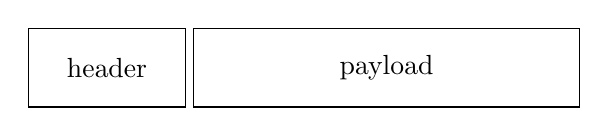
\begin{tikzpicture}
	\draw (0, 0) rectangle (2, 1) node[pos=0.5]{header};
	\draw (2.1, 0) rectangle (7, 1) node[pos=0.5]{payload};
\end{tikzpicture}
	\caption{Datagramme IP}
	\label{fig:datagramme-ip}
\end{figure}

\paragraphe{Modèle en sablier simple}

\begin{tikzpicture}
	\draw
\end{tikzpicture}

\paragraph{Adresses}

\[
	\underbrace{125.255}_{\text{réseau}}.\underbrace{12.1}_{\text{machine}}
\] 

Notation compacte

\[
	/n := (\underbrace{1\cdots 1}_{\text{$n$ fois}} 0 \cdots 0)_2
\] 
\subsubsection{IPv4: problème de pénurie}

\paragraph{IPv6}
 Codé sur 128 bits

 \paragraph{Briser les règles: le NAT}
 Avec un masque: On prend plus de bits pour le réseau et on en laisse moins pour la machine avec un masque 

 \paragraph{Adresses spécifiques}

 \begin{description}
	 \item[bits machine à 0] Adresse réservée au réseau
	\item[bits machine à 1] Adresse de diffusion du réseau
 	\item[0.0.0.0] Route par défaut
	\item[255.255.255.255] Adresse de diffusion sur Internet (ne marche plus :/)
	\item[127.0.0.1] Loopback (même \verb|127.*|)
	\item[10.0.0.0, 172.16.0.0--172.31.0.0, 192.168.0.0--192.168.255.0]  Non routables sur Internet
 \end{description}
 
 


\end{document}
